%! Author = Len Washington III
%! Date = 10/21/2023

% Preamble
\documentclass[19]{cs430lecture}
\usepackage{graphicx}

% Packages

% Document
\begin{document}

%<*Lecture-Activity-19>
\maketitle
\section{Fractional Knapsack Problem}\label{sec:fractional-knapsack-problem}

\begin{enumerate}
    \item Prove that the Fractional Knapsack Problem has optimal substructure.
	\item Try various ``common sense'' greedy approaches that divide the problem into a sub-problem(s) and try to come up with counter-examples or prove the greedy choice is correct using the ``\hyperref[dfn:cut-and-paste]{cut and paste}'' proof.
\end{enumerate}

\section{Huffman Codes Problem}\label{sec:huffman-codes-problem}
Data Encoding Background
\begin{itemize}
	\item Data is a sequence of characters
	\item Fixed Length -- Each character is represented by a unique binary string
	Easy to encode, concatenate the codes together. Easy to decode, break off 3-bit codewords and decode each one.
	\item Variable Length -- Give frequent characters shorter codewords, infrequent characters get long codewords.
	However, how do we decode if the length of the codewords are variable?
	\item Prefix Codes -- No codeword is a prefix of another codeword
	Easy to encode, concatenate the code together.
	Easy to decode, since no codeword is a prefix of another, strip off one bit at a time and match to the unique prefix code
\end{itemize}


Huffman Codes
\begin{itemize}
	\item Are a Data Compression technique using a greedy algorithm to construct an optimal variable length prefix code
	\item Use frequency of occurrence of characters to build an optimal way to represent each character as a binary string
	\item Use a Binary tree method -- 0 means go to left child, 1 means go to right child (not a binary search tree).
	\item Cost of Tree in bits: \[ B(T) = \sum_{\mbox{for all } c\in C} \Call{freq}{c} \times \Call{\hyperref[sec:tree-depth-vs-tree-height]{depth}}{c} \]
\end{itemize}

Example
\begin{table}[H]
    \centering
    \begin{threeparttable}
		\caption{A character-coding problem. A data file of 100,000 characters containes only the characters a--f, with the frequencies indicated. If each character is assigned a 3-bit codeword, the file can be encoded in 300,000 bits. Using the variable-length code shown, the file can be encoded in 224,000 bits.}
		\label{tab:character-encoding-problem}
		\begin{tabular}{lcccccc}
						 & $a$ & $b$ & $c$ & $d$ & $e$ & $f$\\
			\midrule
			Frequency (in thousands)	& 45	& 13	& 12	& 16	& 9		& 5\\
			Fixed-length codeword		& 000	& 001	& 010	& 011	& 100	& 101\\
			Variable-length codeword	& 0		& 101	& 100	& 111	& 1101	& 1100
		\end{tabular}
	\end{threeparttable}
\end{table}

\begin{figure}[H]
	\centering
	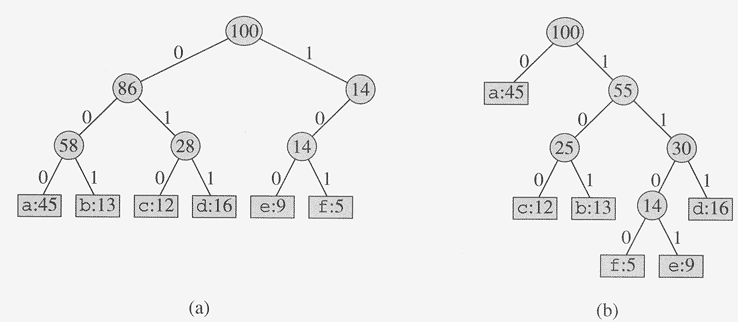
\includegraphics[width=\textwidth]{19.1}
	\caption{Trees corresponding to the coding schemes in Table~\ref{tab:character-encoding-problem}. Each leaf is labeled with a character and its frequency of occurence. Each internal node is labeled with the sum of the frequencies of the leaves in its subtree. \textbf{(a)} The tree corresponding to the fixed-length code $a=000, \dots, f=101$. \textbf{(b)} The tree corresponding to the optimal prefix code $a=0, b=101, \dots, f=1100$.}
	\label{fig:19.1}
\end{figure}
\begin{enumerate}[start=3]
    \item Prove that the Huffman Codes Problem has optimal substructure.
\end{enumerate}

The greedy approach is: Build the tree bottom up by using a minimum priority queue to merge 2 least frequent objects (objects are leaf nodes or other subtrees) together into a new subtree.

\begin{table}[H]
    \centering
    \begin{threeparttable}
		\label{tab:}
		\begin{tabular}{|c|c|}
			\toprule
			\begin{minipage}{0.5\textwidth}
				\begin{figure}[H]
					\centering
					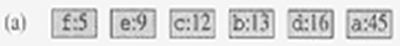
\includegraphics[width=\textwidth]{19.2}
					\label{fig:19.2}
				\end{figure}%
				\begin{figure}[H]
					\centering
					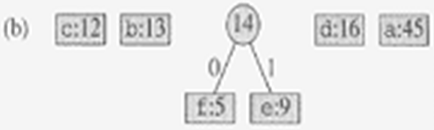
\includegraphics[width=\textwidth]{19.3}
					\label{fig:19.3}
				\end{figure}%
				\begin{figure}[H]
					\centering
					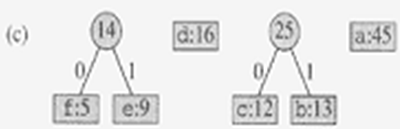
\includegraphics[width=\textwidth]{19.4}
					\label{fig:19.4}
				\end{figure}%
				\begin{figure}[H]
					\centering
					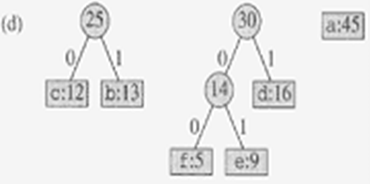
\includegraphics[width=\textwidth]{19.5}
					\label{fig:19.5}
				\end{figure}%
			\end{minipage} &
			\begin{minipage}{0.5\textwidth}
				\begin{figure}[H]
					\centering
					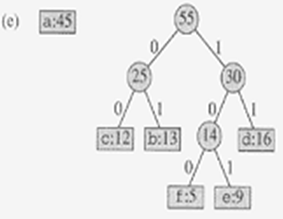
\includegraphics[width=\textwidth]{19.6}
					\label{fig:19.6}
				\end{figure}%
				\begin{figure}[H]
					\centering
					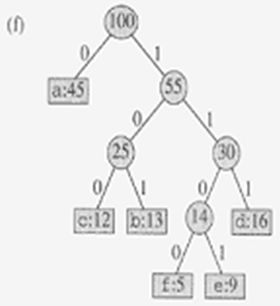
\includegraphics[width=\textwidth]{19.7}
					\label{fig:19.7}
				\end{figure}%
			\end{minipage}\\
			\bottomrule
		\end{tabular}
		\begin{tablenotes}
			\small
			\item Huffman \url{http://www.cs.auckland.ac.nz/software/AlgAnim/huffman.html}
		\end{tablenotes}
	\end{threeparttable}
\end{table}

\begin{enumerate}[start=4]
    \item Proof this greedy algorithm leads to an optimal Huffman Code tree: Build the tree bottom up by using a minimum priority queue to merge 2 least frequent objects (objects are leaf nodes or other subtrees) together into a new subtree.
\end{enumerate}

%</Lecture-Activity-19>

\end{document}